\chapter{Математическое моделирование сложных физических систем}

%=======================



\section{Рамазанов М.К.}



\subsection{Аннотация}

Методом Монте-Карло выполнены исследования магнитных структур основного состояния и термодинамических свойств антиферромагнитной модели Изинга на объемно-центрированной кубической решетке с конкурирующими обменными взаимодействиями. Исследования проведены для соотношения величины обменного взаимодействия следующих и ближайших соседей $r=J_2/J_1=2/3$.

Получены все возможные магнитные структуры основного состояния для данного соотношения обменных взаимодействий. Показано, что при значении $r=2/3$ конкуренция обменных взаимодействий не приводит к возникновению фрустрации и вырождению основного состояния. На основе гистограммного метода анализа данных показано, что в исследуемой модели при $r=2/3$ наблюдается фазовый переход второго рода.


\subsection{Введение}

В настоящее время продолжается активное исследование магнитных состояний, фазовых переходов (ФП), критических и термодинамических свойств в спиновых системах с конкурирующими обменными взаимодействиями. Конкуренция обменного взаимодействия может привести к возникновению в системе эффектов фрустрации. Наличие фрустраций в системе может привести к целому ряду изменений свойств фундаментального характера \cite{ph1_1,ph1_2,ph1_3}. Учет антиферромагнитных взаимодействий следующих ближайших соседей в классической трехмерной модели Изинга приводит к вырождению основного состояния, появлению различных фаз, ФП и аномалий критических и термодинамических свойств \cite{ph1_4}.

В данной работе, нами на основе метода Монте-Карло (МК) проведено исследование ФП, магнитной структуры основного состояния и термодинамических свойств антиферромагнитной модели Изинга на объемно-центрированной кубической решетке для соотношения величины обменного взаимодействия следующих и ближайших соседей $r=J_2/J_1=2/3$ ($J_1$ и $J_2$ --- константы обменного взаимодействия ближайших и следующих за ближайшими соседей, соответственно).

Литературные данные по исследованию этой модели различными методами свидетельствуют, что для данной модели имеет место ФП второго рода. Эти данные показывают, что учет взаимодействий следующих ближайших соседей в системе может привести к смене ФП. Результаты, имеющиеся в литературе свидетельствуют, что данная модель имеет некоторые особенности критического и термодинамического поведения вблизи точки пересечения трех различных фаз на фазовой диаграмме. Исследование этих особенностей в самой точке пересечения этих фаз на сегодняшний день не проведено. Исходя из этого, целесообразно более подробно исследовать особенности, наблюдающиеся для этой модели в точке пересечения трех различных фаз. Эти особенности могут быть связаны со структурой основного состояния, которая до сих пор является малоизученной.

В связи с этим, в данной работе, нами предпринята попытка исследовать ФП, термодинамическое поведение системы и магнитную структуру основного состояния в точке пересечения трех различных фаз этой модели. Исследование этой модели на основе современных методов и идей позволит получить ответ на ряд вопросов, связанных со структурой основного состояния, с характером и природой ФП спиновых систем с конкурирующими обменными взаимодействиями.



\subsection{Результат исследования}



Получена фазовая диаграмма зависимости критической температуры от величины взаимодействия следующих ближайших соседей (рис. \ref{phys1-pic-1}). На диаграмме видно, что в точке $r=2/3$ пересекаются три различные фазы: $AF1$ -- антиферромагнитная, $PM$ -- парамагнитная и $AF2$ -- антиферромагнитная $2$-го типа. На фазовой диаграмме черными и светлыми стрелками изображены направления спинов во всех подрешетках. Обнаружены все возможные магнитные структуры основного состо-яния, наблюдаемые в данной модели. Вдоль вертикальной пунктирной линии, соответствующей значению $r=2/3$ на диаграмме сосуществуют все шесть структур одновременно.

\begin{figure}[H]
	\centering
	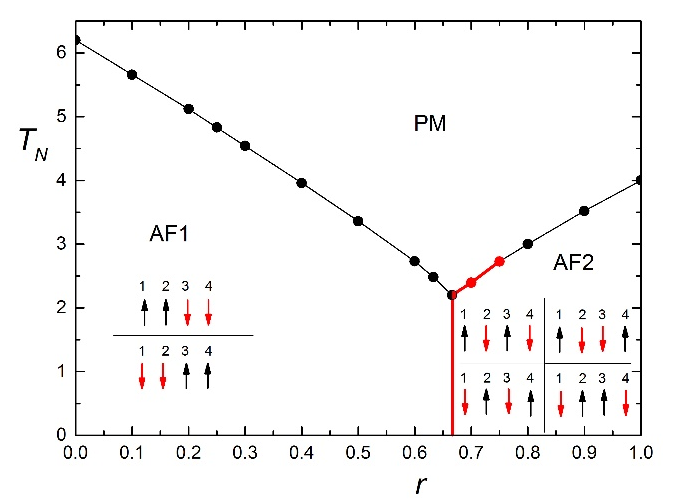
\includegraphics[width=0.5\linewidth]{content/sections/images/phys1-1}
	\caption{Фазовая диаграмма антиферромагнитной модели Изинга на ОЦК решетке.}
	\label{phys1-pic-1}
\end{figure}

Впервые на диаграмме обнаружена узкая область $(2/3 < r \leq 3/4)$, где переход из антиферромагнитной фазы в парамагнитную является переходом первого рода. Обнаружено, что при значении $r=2/3$ конкуренция обменных взаимодействий не приводит к возникновению фрустрации и вырождению основного состояния. Показано, что в исследуемой модели при $r = 2/3$ наблюдается фазовый переход второго рода.






\subsection{Заключение}



Исследование фазовых переходов, термодинамических свойств и магнитной структуры основного состояния в антиферромагнитной модели Изинга на объемно-центрированной кубической решетке с конкурирующими обменными взаимодействиями выполнено с использованием репличного алгоритма и алгоритма Ванга -- Ландау метода Монте-Карло. Показано, что при значении $r=2/3$ конкуренция обменных взаимодействий не приводит к возникновению фрустрации. На основе гистограммного метода анализа данных показано, что для значения $r=2/3$ в данной модели наблюдается фазовый переход второго рода.


